\documentclass{beamer}


\usetheme{Madrid}


\title{From Cloud to Edge: Seamless Software
	Migration at the Era of the Web of Things}
\author{Michele Beccari 856608}
\date{2023}

\begin{document}
	
	\begin{frame}
		\titlepage
	\end{frame}
	
	\begin{frame}[allowframebreaks]{Indice}
		\tableofcontents
	\end{frame}
	
	\section{Introduzione}
	
	
	\begin{frame}{Introduzione}
		\begin{block}{Lo standard Web of things}
				Standard promosso dal W3C per progettare sistemi IoT interoperabili in grado di gestire l’eterogeneità delle piattaforme software
				e dei dispositivi
		\end{block}
		\begin{exampleblock}{Cosa consente di fare?}
			Consente la creazione di scenari di IoT caratterizzati da una moltitudine di Web Things (WTs)
			che comunicano secondo delle interfacce software ben definite
		\end{exampleblock}
		\begin{alertblock}{Tuttavia...}
			presume un’allocazione statica delle WTs agli host e non è in grado di gestire
			la dinamicità intrinseca degli ambienti IoT per quanto riguarda le variazioni del carico di rete e
			computazionale.
		\end{alertblock}
	\end{frame}

	\begin{frame}{Introduzione}
		\begin{block}{Obbiettivo del paper}
			Vogliamo estendere il paradigma WoT al deployment nel continuo cloud-edge. In
			questo modo potremmo supportare un’orchestrazione dinamica e la mobilità delle WTs su tutte le
			risorse di calcolo disponibili.
		\end{block}
		\begin{block}{Migratable WoT (M-WoT)}
			Vogliamo sfruttare lo
			standard WoT e in particolare la sua capacità di standardizzare le interfacce software delle WT per
			proporre il concetto di Migratable WoT (M-WoT ).
			In un Migratable WoT le WT sono allocate senza soluzione di continuità agli host a seconda delle loro
			interazioni dinamiche
		\end{block}
	\end{frame}




	\begin{frame}{Introduzione}
	\begin{block}{Gli ambienti IoT sono ambienti dinamici}
		Le applicazioni software IoT devono adattarsi a cambiamenti rapidi: 
			\begin{enumerate}
			\item nell'utilizzo di banda
			\item nell'utilizzo di risorse di calcolo
			\item nel numero di dispositivi connessi
			\item nei requisiti del servizio
		\end{enumerate}
	\end{block}
	\begin{block}{Per questo motivo}
	Diverse piattaforme per l’IoT forniscono uno strato di adattamento supportando la mobilità senza
	soluzione di continuità lungo i nodi di un continuo cloud-edge
	\end{block}
	\end{frame}


	\begin{frame}{Introduzione}
	\begin{block}{Inoltre}
		i dispositivi IoT mobili che generano stream di dati mutevoli nello spazio e nel
		tempo spingono la ricerca verso delle architetture di calcolo flessibili in grado di auto configurarsi per
		soddisfare la qualità del servizio (QoS) per le applicazioni utente.
	\end{block}
	\begin{block}{Per questo motivo}
		Diverse piattaforme per l’IoT forniscono uno strato di adattamento supportando la mobilità senza
		soluzione di continuità lungo i nodi di un continuo cloud-edge
	\end{block}
	\end{frame}


	\begin{frame}{Introduzione}
	\begin{block}{MEC}
		L'architettura mobile edge computing (MEC) cerca di eseguire i processi in prossimità delle sorgenti dati.\\
		Questo avviene utilizzando:
		\begin{itemize}
			\item Tecniche di mobilità di container e/o virtual machine
			\item Politiche di migrazione guidate dalla mobilità fisica dei dispositivi IoT
		\end{itemize}
	\end{block}
	\end{frame}


	\begin{frame}{Introduzione}
	\begin{alertblock}{Problemi di interoperabilità}
		La maggior parte degli ambienti IoT sono
		caratterizzati dall’eterogeneità dei componenti hardware e software e dalla dinamicità delle loro inter-
		azioni.
	\end{alertblock}
	\begin{exampleblock}{Possibili soluzioni}
		\begin{itemize}
			\item Nuove opportunità di business possono nascere offrendo soluzioni che consentono a
			sistemi IoT diversi di comunicare fra loro.
			\item Gli ecosistemi cloud possono mitigare alcuni dei
			problemi di interoperabilità con l’utilizzo di tecnologie web (es. api REST, JSON , web sockets ecc...)
		\end{itemize}
	\end{exampleblock}
	\begin{alertblock}{Ma...}
		Spesso le soluzioni si basano spesso su architetture ”a silo” con un vendor lock-in esplicito o implicito.
	\end{alertblock}
	\end{frame}

	\section{Lo standard WoT del W3C}
	\subsection{Lo standard WoT del W3C - Che cos'è}
	\begin{frame}{Lo standard WoT del W3C - Che cos'è}
	\begin{exampleblock}{Che cos'è}
		Standard pubblico nato nel 2015 con l’obbiettivo di definire un insieme di
		standard di riferimento che consentisse l’interoperabilità fra diversi sistemi IoT.
	\end{exampleblock}
	\begin{exampleblock}{Le novità}
		Definizione della Web thing (WT), che rappresenta l’astrazione di un’entità
		fisica o virtuale.  \\
		I metadati e l’interfaccia dell'entità possono essere descritti formalmente da una WoT thing
		description (TD)
	\end{exampleblock}
	\begin{block}{\textit{Thing description}}
		Interfaccia standard per i
		componenti IoT (fisici o virtuali) che definisce formalmente le capacità
		e le potenzialità delle web thing.
	\end{block}
	\end{frame}



	\begin{frame}{Lo standard WoT del W3C - Architettura}
		\begin{columns}[T]
			\begin{column}{0.5\textwidth}
				\begin{block}{L'architettura}
					L'architettura di una WT comprende quattro blocchi di nostro interesse:
					\begin{itemize}
						\item Interaction affordances
						\item Security Configuration
						\item Protocol bindings
						\item Behaviour
					\end{itemize}
				\end{block}
			\end{column}
			\begin{column}{0.5\textwidth}
				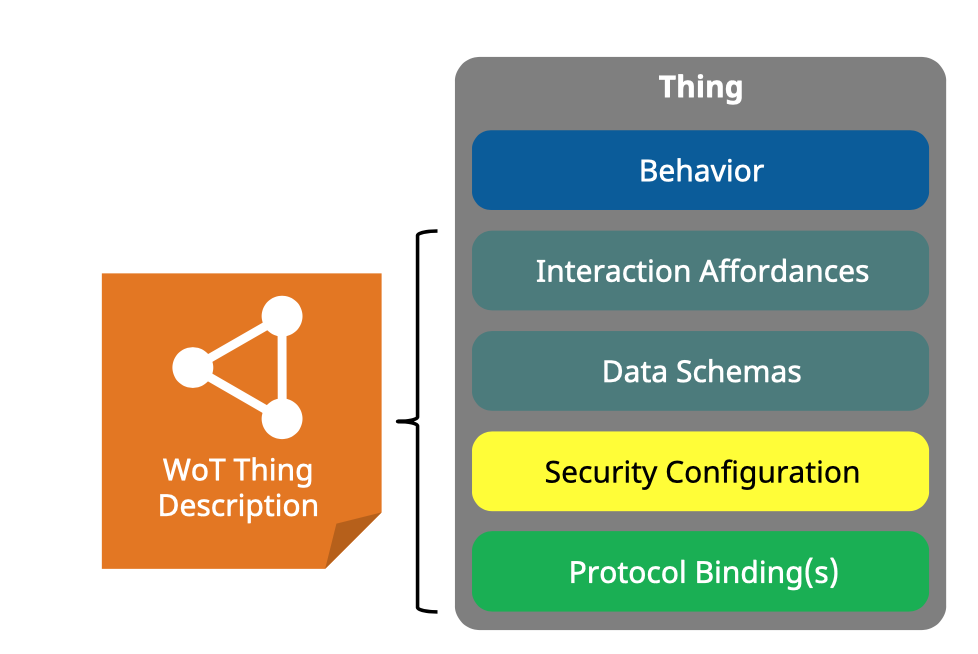
\includegraphics[width=\textwidth]{./images/3.png}
			\end{column}
		\end{columns}
	\begin{block}{I blocchi della WT}
		I primi tre blocchi sono inclusi nella TD: l’ultimo può essere descritto come una sequenza di metadati
		standardizzati comprensibili dalla macchina che consentono ai consumatori di scoprire ed interpretare
		le capacità di una WT per poterci interagire.
	\end{block}
	
	\end{frame}

	\begin{frame}{Lo standard WoT del W3C - Architettura}
	\begin{block}{In dettaglio}
		I primi tre blocchi sono inclusi nella TD: l’ultimo può essere descritto come una sequenza di metadati
		standardizzati comprensibili dalla macchina che consentono ai consumatori di scoprire ed interpretare
		le capacità di una WT per poterci interagire.
	\end{block}
 \begin{block}{Interaction Affordances}
	Fornisce un modello astratto di come i consumatori possono interagire con la WT, in termini di proprietà, azioni ed eventi.
\end{block}

\begin{block}{Protocol Bindings}
	Definiscono la mappatura tra le affordances astratte e le strategie di rete (protocolli) che possono essere utilizzate per interagire con la WT.
\end{block}


	
\end{frame}

\begin{frame}{Lo standard WoT del W3C - Architettura}
	\begin{block}{Security Configuration}
		Definisce i meccanismi di controllo dell'accesso alle affordances.
	\end{block}
	\begin{block}{Behaviour}
		 Consiste nelll’implementazione della WT,incluse le affordances (il codice delle azioni)
	\end{block}
	\begin{block}{Servient}
		Runtime all'interno del quale vengono eseguiti tutti i blocchi della WT, può operare in modalità server o in modalità client.
	\end{block}
\end{frame}

\subsection{Lo standard WoT del W3C - Servient}
\begin{frame}{Lo standard WoT del W3C - Servient}
	\begin{columns}[T]
		\begin{column}{0.45\textwidth}
			\begin{block}{Modalità server}
				Il servient hosta ed \textit{espone} le cose, ovvero crea un oggetto a run-time che serve le richieste verso la WT che sta hostando (come accedere alle proprietà esposte, alle azioni e agli eventi)
			\end{block}
		\end{column}
		\begin{column}{0.45\textwidth}
			\begin{block}{Modalità client}
				Il servient \textit{consuma} le cose. In questo caso il servient  processa le TD, genera una rappresentazione a runtime chiamata la "consumed thing" e la rende disponibile ai client che stanno interagendo con la WT remota.
			\end{block}
		\end{column}
	\end{columns}
\end{frame}



\subsection{Lo standard WoT del W3C - Limiti e obbiettivi}
	\begin{frame}{Lo standard WoT del W3C - Limiti e obbiettivi}
		\begin{alertblock}{I limiti}
			L’implementazione di riferimento del WoT
			non supporta la mobilità dei componenti software fra i nodi del cloud o dell’edge
		\end{alertblock}
		\begin{exampleblock}{Gli obbiettivi del paper}
			Vogliamo estendere le funzionalità del WoT per gli ambienti
			IoT supportando l’orchestrazione dinamica e la mobilità delle WT’s fra tutte le risorse computazionali
			disponibili di tutto lo spettro IoT (nodi dell’edge/fog/cloud).
			\begin{itemize}
				\item Come rendere possibile la migrazione senza soluzione di continuità di una WT fra due nodi?
				\item Come ottimizzare le performance di un deployment WoT orchestrando le allocazioni delle WT nel continuo cloud edge?
			\end{itemize}
		\end{exampleblock}
	\end{frame}

\section{M-WOT}


\subsection{M-WOT - migrazione}
\begin{frame}{M-WOT - migrazione}
\begin{block}{Migrazione di una WT}
Definiamo la migrazione WT come la capacità di associare dinamicamente un WT a diversi nodi, stoppando l'esecuzione al nodo sorgente e riprendendola al nodo di destinazione. \\
\end{block}
\begin{block}{Stato della WT}
	Presumiamo che il processo di migrazione sia stateful, ovvero lo stato interno di una WT e la su TD doverebbero essere spostati e aggiornati insieme al codice. \\
\end{block}
\begin{block}{In particolare}
	Tutti i valori delle Properties e le informazioni che descrivono il contesto di  computazione della WT doverebbero essere considerati parte dello stato quindi migrati.
\end{block}

\end{frame}

\subsection{M-WOT - scenario d'esempio}
\begin{frame}{M-WOT - scenario d'esempio}
	\begin{columns}
		\begin{column}[c]{0.5\textwidth}
			\begin{block}{Lo scenario}
				Consideriamo uno scenario distribuito composto da un insieme di nodi di calcolo distribuiti lungo
				tutto lo stack dello spettro IoT (dall’edge al cloud) come mostrato nella figura a lato; ogni nodo è abilitato
				al WoT, ovvero puà hostare uno o più servient  e ogni
				servient contiene una singla WT in stato di esecuzione.
			\end{block}
		\end{column}
		\begin{column}[c]{0.5\textwidth}
			\centering
			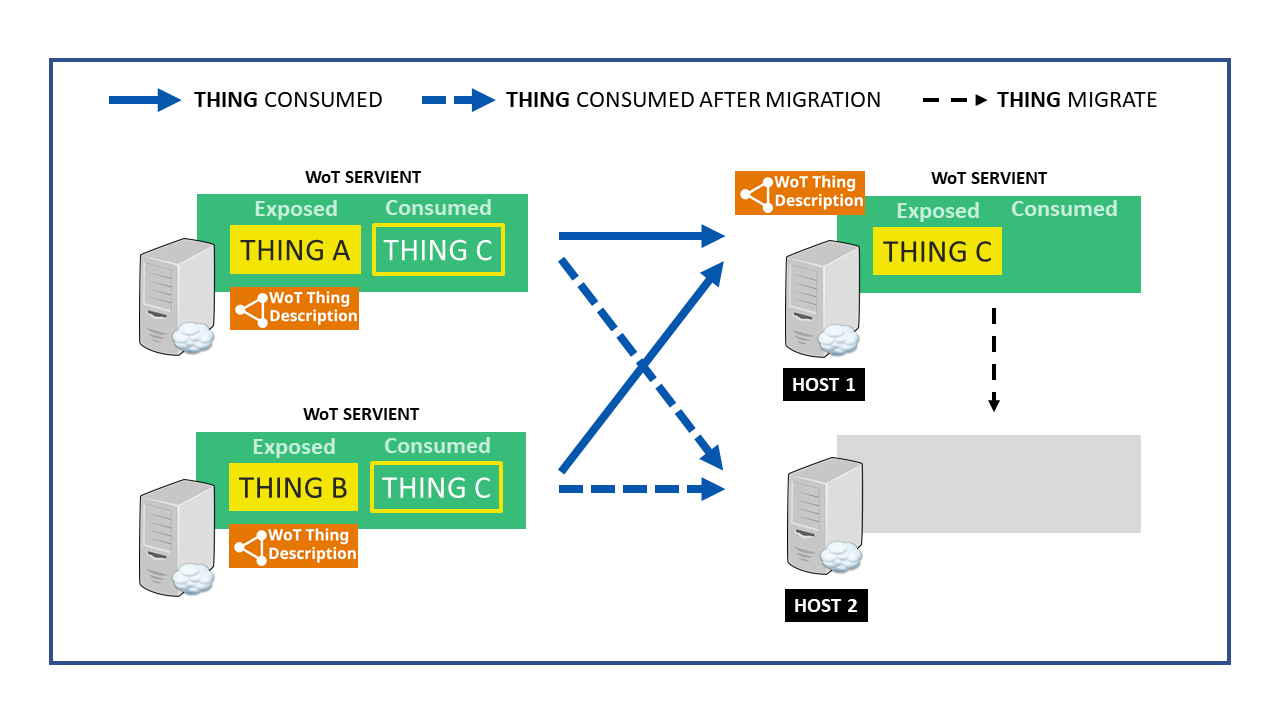
\includegraphics[width=\textwidth]{./images/4.png}
		\end{column}
	\end{columns}
\end{frame}



\subsection{M-WOT - challenge}

\begin{frame}{M-WOT - challenge}
	\begin{alertblock}{challenge: Thing handoff management}
		Se una WT migra su un altro nodo, tutte le altre WTs che la stavano consumando devono essere notificare per poter aggiornare i loro oggetti consumati e puntare al nuovo indirizzo della TD. \\
	\end{alertblock}
\end{frame}


\begin{frame}{M-WOT - challenge}
	\begin{columns}
		\begin{column}[c]{0.5\textwidth}
			\begin{block}{Thing handoff management}
				Nella figura entrambe le WT A e B stanno consumando la WT C;\ \
				La WT C verrà migrata dall'host 1 all'host 2 in un'istante futuro. \\

			\end{block}
		\end{column}
		\begin{column}[c]{0.5\textwidth}
			\centering
			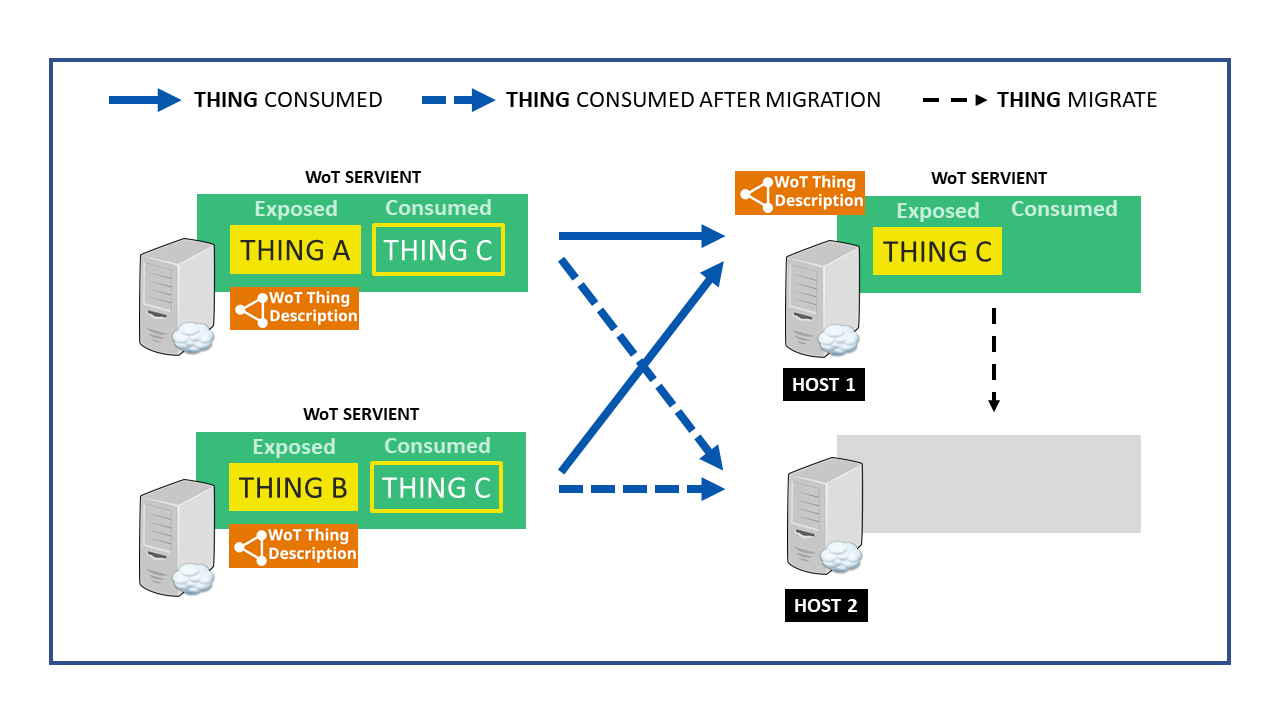
\includegraphics[width=\textwidth]{./images/4.png}
		\end{column}
	\end{columns}
	\begin{block}{Quindi}
		Una procedura di signalling adeguata deve essere effetuata per informare A e B di quando l'attivazione della WT C sull'host 2 è stata completata, in modo tale che possano consumare nuovamente la TD della WT C. \\
	\end{block}
	\begin{alertblock}{Inoltre}
		il processo di migrazione introduce un intervallo di handoff durante il quale la WT C potrebbe non essere in grado di processare le invocazioni remote dalla WT A e B.
	\end{alertblock}
\end{frame}

\subsection{M-WOT - advantage}
\begin{frame}{M-WOT - advantage}
	\begin{block}{L'idea}
		Un framework per la migrazione WoT potrebbe supportare la mobilità di gruppi di componenti software  come conseguenza delle dipendenze attive di dati (le interazioni ) fra le WT \\
	\end{block}
	\begin{block}{Grazie allo standard WoT}
		Ogni WT espone le proprie affordances attraverso la TD in maniera standardizzata
	\end{block}
	\begin{block}{Questo constente di}
		Costruire un grafico delle dipendenze real-time fra tutte le WT di un sistema WoT distribuito.
	\end{block}
\end{frame}

\subsection{M-WOT - advantage}
\begin{frame}{M-WOT - advantage}
	\begin{block}{Utilizzando il grafo}
		Diventa possibile progettare policy di allocazione che determinano migrazioni
		di gruppo di sottoinsiemi di WTs che interagiscono fra di loro per massimizzare la località dei
		dati. \\
	\end{block}
\end{frame}


\subsection{M-WOT - architettura}
\begin{frame}{M-WOT - architettura}
	\begin{columns}
		\begin{column}[c]{0.5\textwidth}
			\begin{block}{I componenti del deployment}
				 Consideriamo un insieme di servients del WoT deployati su diversi nodi, ogni servient hosta esattamente una WT.
			\end{block}
		\begin{block}{Le differenze}
			In maniera differente rispetto ad un deployment WoT legacy, che si presume essere statico, il M-Wot consente la mobilità delle WT fra nodi diversi.
		\end{block}
		\end{column}
		\begin{column}[c]{0.45\textwidth}
			\centering
			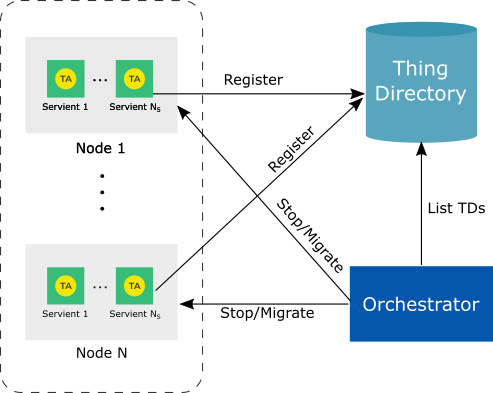
\includegraphics[width=\textwidth]{./images/7.png}
		\end{column}
	\end{columns}
\end{frame}

\begin{frame}{M-WOT - architettura}
	\begin{columns}
		\begin{column}[c]{0.5\textwidth}
			\begin{block}{Per gestire la mobilità}
			 	Il M-WoT offre due nuovi componenti, che non migrano.
			 	\begin{itemize}
			 		\item L'orchestrator
			 		\item Thing directory
			 	\end{itemize}
			\end{block}
		\end{column}
		\begin{column}[c]{0.45\textwidth}
			\centering
			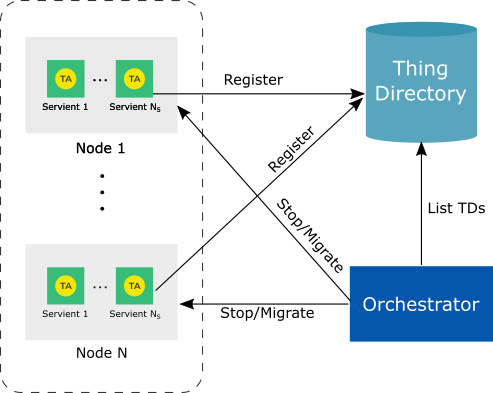
\includegraphics[width=\textwidth]{./images/7.png}
		\end{column}
	\end{columns}
\end{frame}


\subsection{M-WOT - thing directory}
\begin{frame}{M-WOT - thing directory}
	\begin{block}{Il thing directory }
		Serve come registro delle risorse del M-WoT, ovvero delle thing descriptors attive.\\
		Svolge due funzionalità:
		\begin{itemize}
			\item Servizio di discovery
			\item Supporta le notifiche push
		\end{itemize}
	\end{block}
	\begin{block}{Servizio di discovery}
		Quando viene interrogato dai client (soprattutto dall'orchestrator) ritorna la lista dei TD che rispettano i parametri di interrogazione
	\end{block}
	\begin{block}{Supporto alle notifiche push}
		Invia notifiche verso i servient, quando specifici eventi di sistema sono rilevati (ad esempio quando una WT comleta la procedura di handoff.)
	\end{block}
\end{frame}

\subsection{M-WOT - orchestrator}
\begin{frame}{M-WOT - orchestrator}
	\begin{block}{L' orchestrator}
		Costituisce il componente core dell'architettura M-WoT.
	\end{block}
	\begin{block}{Per tutta la vita del sistema}
		\begin{enumerate}
			\item Usa la TDir per recuperare la lista dei servient attivi (ovvero delle loro TD)
			\item Interroga ogni servient attraverso la sua interfaccia WoT per raccogliere statistiche live (es. uso della CPU o traffico di rete)
			\item Basandosi sui valori delle metriche ricevute e sulle politiche di ottimizzazioni in uso determina il piano di allocazione dei servient sui nodi.
			\item Trasferisce il piano di allocazione ad un layer sottostante (esterno al M-Wot) chiamato in genere  il \textit{Migration substrate} (incaricato di implementare la mobilità fisica del software fra i nodi sorgenti e i nodi di destinazione)
		\end{enumerate}
	\end{block}
\end{frame}

\subsection{M-WOT - orchestrator - struttura interna}
\begin{frame}{M-WOT - orchestrator - struttura interna}
	\begin{columns}
	\begin{column}[c]{0.5\textwidth}
	\begin{block}{La struttura interna}
	Per favorire l'estensibilità della piattaforma la struttura dell'orchestrator è stata divisa in tre sottomoduli principali
\end{block}
	\end{column}
	\begin{column}[c]{0.35\textwidth}
		\centering
		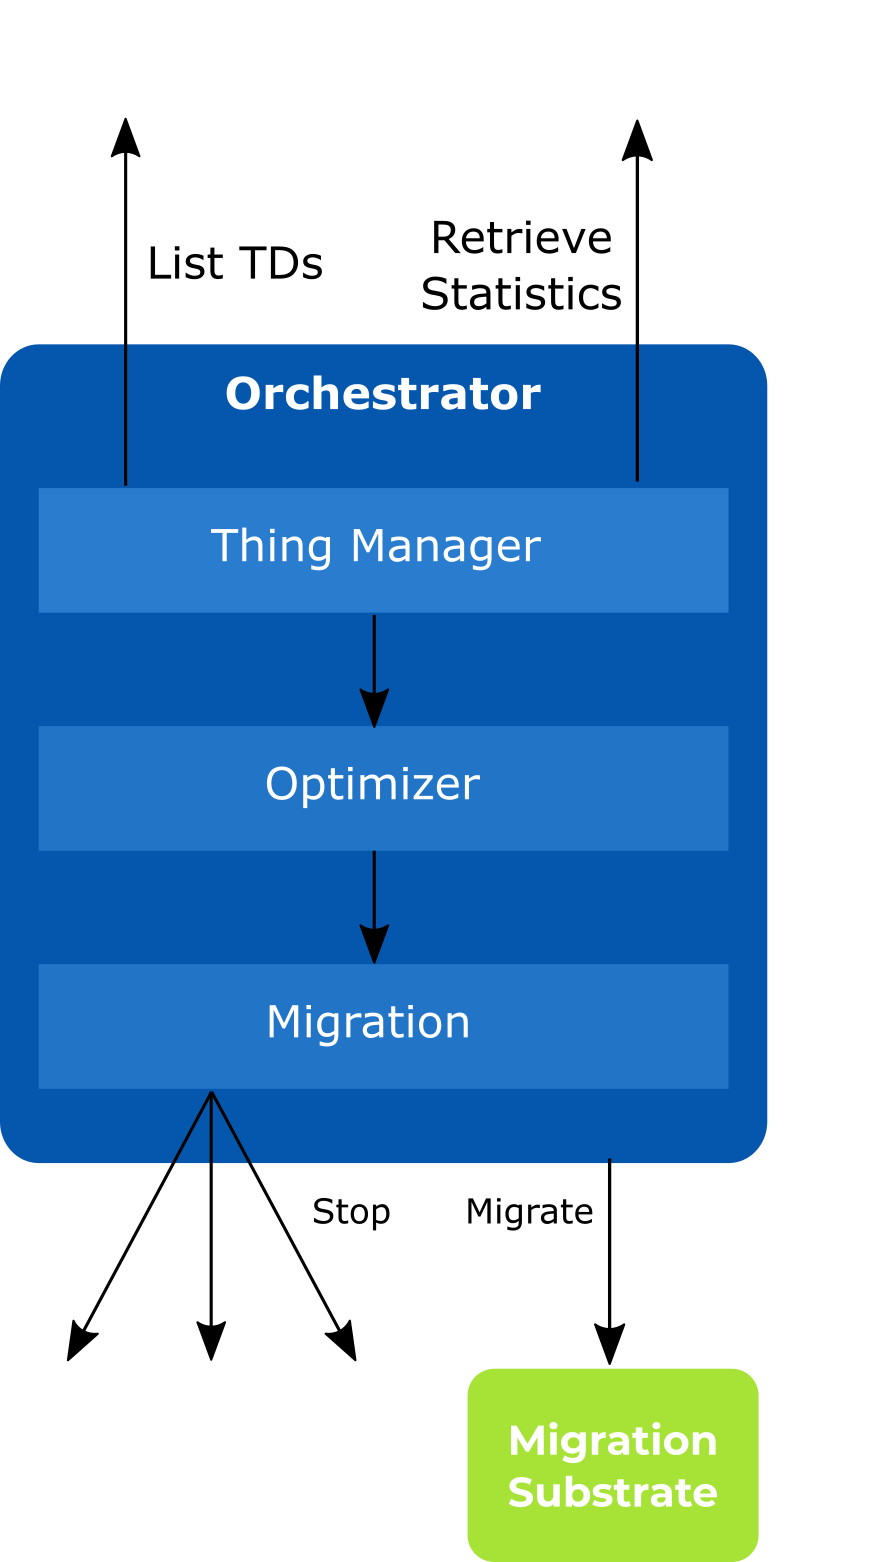
\includegraphics[width=\textwidth]{./images/8.png}
	\end{column}
\end{columns}
\end{frame}


\subsection{M-WOT - orchestrator - struttura interna}
\begin{frame}{M-WOT - orchestrator - struttura interna}
	\begin{columns}
		\begin{column}[c]{0.6\textwidth}
			\begin{block}{Thing manager}
				Polla periodicamente i dati dalla TDir per gestire la lista dei servient attivi e le rispettive TD.
			\end{block}
			\begin{block}{Optimizer}
				Esegue la policy di allocazione per i servient.
			\end{block}
			\begin{block}{Migration}
			Riceve il piano di deployment dell'optimizer e implementa le procedure di handoff per i servient.
			\end{block}
		\end{column}
		\begin{column}[c]{0.35\textwidth}
			\centering
			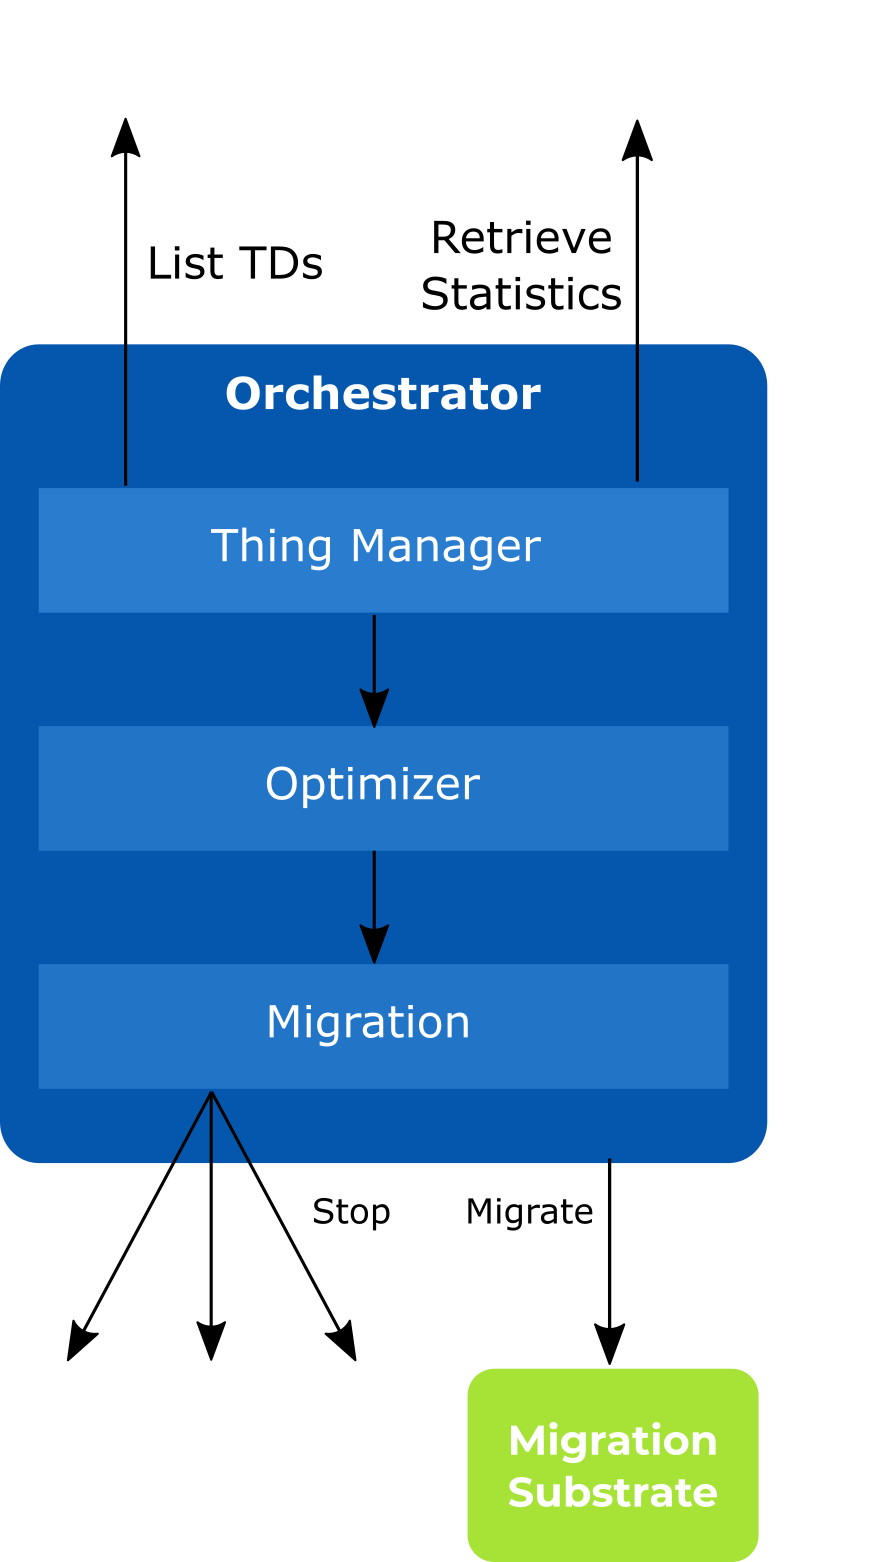
\includegraphics[width=\textwidth]{./images/8.png}
		\end{column}
	\end{columns}
\end{frame}

\subsection{M-WOT - servient}
\begin{frame}{M-WOT - servient}
	\begin{columns}
	\begin{column}[c]{0.6\textwidth}
		\begin{block}{Servient M-WoT}
			Presenta modifiche al runtime servient per fornire all'optimizer dati in tempo reale sulle performance del sistema
		\end{block}
		\begin{block}{Strato di API di monitoraggio}
			Esegue la policy di allocazione per i servient.
		\end{block}
		\begin{block}{Migration}
			Riceve il piano di deployment dell'optimizer e implementa le procedure di handoff per i servient.
		\end{block}
	\end{column}
	\begin{column}[c]{0.35\textwidth}
		\centering
		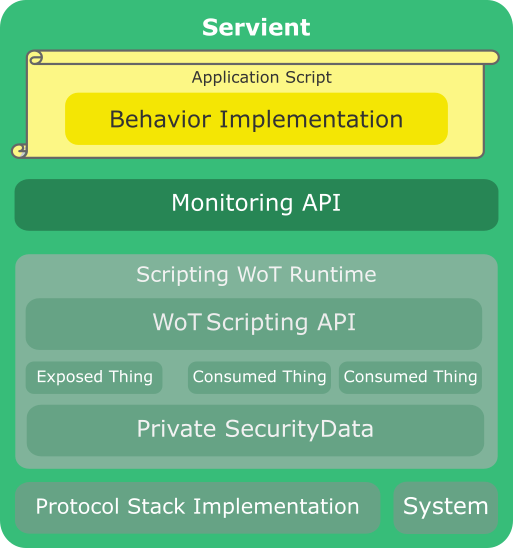
\includegraphics[width=\textwidth]{./images/9.png}
	\end{column}
\end{columns}
\end{frame}



\begin{frame}{M-WOT - servient}
	\begin{block}{In particolare}
	Il nuovo strato di API di monitoraggio è incaricato di intercettare le invocazione all'api di scripting e di generare periodicamente dei \textit{Thing Report} (Trs).
	\end{block}
	\begin{block}{\textit{Thing Report} (TR)}
	Snapshot dell'esecuzione corrente del servient che contengono i valori delle metriche del servient richieste dall'optimizer
	\end{block}
	
\end{frame}


\subsection{M-WOT - esempio di migrazione}
\begin{frame}[allowframebreaks]{M-WOT - esempio di migrazione}
\begin{block}{Consideriamo due WT/Servient}
	Rispettivamente $T_A$/$S_A$ e $T_B$/$S_B$ (con $T_A$ in esecuzione su $S_A$ e $T_B$ su $S_B$) hostati sui nodi $N_1$ ed $N_2$
\end{block}
\begin{block}{Assumiamo che}
	$T_B$ abbia consumato $T_A$ e che stia leggendo periodicamente alcune delle sue proprietà.
\end{block}
\begin{block}{All'istante $t$ }
	Il thing manager interroga $S_A$ e $S_B$ per raccogliere le $TR$
\end{block}
\begin{block}{Successivamente}
	L'optimizer viene eseguito: una nuova allocazione viene prodotta dove $T_A$ deve essere spostato sul nodo $N_2$. 
\end{block}

\begin{block}{È necessario migrare $T_A$ da $N_1$ ad $N_2$}
	\begin{enumerate}
		\item L'esecuzione corrente di $T_A$ viene stoppata dall'orchestrator
		\item Il contesto applicativo di $T_A$ è salvato come metadati all'intendo di TDir
		\item L'orchestrator invia una richiesta al migration substrate per far muovere $T_A$/$S_A$ al nodo di destinazione ($N_2$)
	\end{enumerate}
\end{block}

\pagebreak

\begin{block}{Dopo che $S_A$ è stato rigenerato su $N_2$}
	\begin{enumerate}
		\item Registra la sua nuova TD (con gli indirizzi di rete delle sue affordances aggiornate) nel TDir
		\item Interroga la TDir per recuperare il contesto della $T_A$, quest'ultimo viene deserializzato e iniettato come oggetto globale nello script applicativo della $T_A$
		\item $T_A$ inizia il processo di inizializzazione e si espone facendo partire la registrazione della propria TD all'interno della TDir
		\item $T_A$ riprende nello stato in cui era prima di essere stoppata ed è considerata completamente migrata.
	\end{enumerate}
\end{block}

\pagebreak

\begin{block}{Dopo che $S_A$ è stato rigenerato su $N_2$}
	\begin{enumerate}
		\item Registra la sua nuova TD (con gli indirizzi di rete delle sue affordances aggiornate) nel TDir
		\item Interroga la TDir per recuperare il contesto della $T_A$, quest'ultimo viene deserializzato e iniettato come oggetto globale nello script applicativo della $T_A$
		\item $T_A$ inizia il processo di inizializzazione e si espone facendo partire la registrazione della propria TD all'interno della TDir
		\item $T_A$ riprende nello stato in cui era prima di essere stoppata ed è considerata completamente migrata.
	\end{enumerate}
\end{block}

\begin{block}{Infine}
	\begin{enumerate}
		\item La TDir invia una notifica a $T_B$ riguardo la procedura di handoff.
		\item $T_B$ recupera la nuova TD di $T_A$ dalla TDir e la consuma di nuovo per poter puntare alla posizione del servizio aggiornata
		\item $T_B$ ricomincia ad interagire con $T_A$ e ad accedere alle sue affordances.
	\end{enumerate}
\end{block}

\end{frame}

\section{Migration Policy}
\subsection{Migration Policy - scopo}
\begin{frame}{Migration Policy - scopo}
	\begin{block}{Scopo}
		Vogliamo rappresentare formalmente le operazioni dell'optimizer come problema di ottimo multi obbiettivo
	\end{block}
	\begin{block}{Come?}
		Consideriamo un processo di ottimizzazione a due passaggi che considera:
		\begin{itemize}
			\item il problema del load balancing (ovvero quanto carico ha ogni host)
			\item l'overhead delle comunicazioni di rete (ovvero quanti dati vengono scambiati fra gli host)
		\end{itemize}
	\end{block}
\end{frame}

\subsection{Migration Policy - formulazione del problema}
\begin{frame}[allowframebreaks]{Migration Policy - formulazione del problema}
	\begin{block}{Scenario}
		Consideriamo un generico deployment WoT con $N_{WT}$ WT attive.
	\end{block}
	\begin{block}{Il sistema evolve nel tempo}
		Su una serie di time-slot $T = \{t_0, t_1...\}$; ogni slot ha una durata di $t_{slot}$ secondi ed è uguale all'intervallo fra le esecuzioni consecutive della policy di migrazione
	\end{block}
	\begin{block}{Il sistema comprende un insieme di WT}
		Poniamo \[WT = \{ wt_1, wt_2, ... wt_{N_{WT}} \}\] come l'insieme delle WT, che possono essere eterogenee in termini di modello dei dati (es. le affordances).
	\end{block}
	\begin{block}{Le WT offrono una serie di affordances}
		Senza perdere in generalità poniamo \[A_i = \{a_i^1, a_i^2, ... a_i^{N_{A_i}}\}\] Ovvero le affordances esposte dalla $wt_i$ nella sua TD, ogni affordance può rappresentare una proprietà, un'azione oppure un evento.
	\end{block}
	\begin{alertblock}{Le affordances sono un insieme statico}
		Presumiamo che $A_i$ sia statico, ovvero $wt_i$ non può aggiornare la propria $TD$ a runtime (es. non può definire nuove proprietà)
	\end{alertblock}
	\pagebreak
	\begin{block}{Il sistema comprende un insieme di host}
		Poniamo $H$ l'insieme dei nodi di host. \[H = \{h_1, h_2, ... h_{N_H}\}\] e assumiamo che i nodi siano eterogenei in termini di hardware.
	\end{block}
	\begin{alertblock}{Gli host sono eterogenei fra loro}
		Senza perdere in generalità modelliamo la diversa potenza di calcolo attraverso un'indice di potenza computazionale \[\gamma(h_l), \forall h_l \in H\] che astrae i dettagli dell'hardware ed è definito come il numero massimo di things che possono essere eseguite sull'host
	\end{alertblock}
	\pagebreak
	
	\begin{block}{L'allocazione dei servient agli host}
	 È definita dalla funzione policy 
	 \[
	 	P : WT \times T \rightarrow H;
	 \]
	Per ogni WT $wt_i$ il valore $P(wt_i, tk) = h_m$ specifica la macchina (ovvero $h_m$) che la sta hostando all'istante di tempo $t_k$.
	\end{block}
	\begin{block}{Basandosi sull'output della policy di allocazione}
		L'insieme \[PT_{m,k} \subseteq WT\] denota la lista delle WT che sono hostate dall'host $h_m$ nel time slot $t_k$, ovvero \[PT_{m,k} = \{ wt_i \in WT | P(wt_i, t_k) = h_m \}\]. \\
	\end{block}
	\begin{block}{Ogni WT $wt_i$ può interagire con un altra WT $wt_j$ se prima la consuma}
			Questo cosa è modellata con l'assunzione che, in ogni time slot $t_k$, $wt_i$ può inviare una lista di richieste \[R_{i,j,k} = \{ r^1_{i,j,k}, r^2_{i,j,k} ...  \}\] alla $wt_j$ consumata.
	\end{block}

	\begin{block}{L'implementazione di ogni richiesta $r^y_{i,j,k}$ comporta dello scambio di dati fra le WT $wt_i$ e $wt_j$}
		definiamo \[B(r^y_{i,j,k})\] come i dati scambiati (in byte) fra le due WT, includendo sia gli eventuali parametri passati da $wt_i$ a $wt_j$ sia eventuali valori di ritorno da $wt_j$ a $wt_i$.
	\end{block}

	\begin{block}{Carico totale}
		Denotiamo con \[B(i, j, k) = \sum_{}^{} B(r^y_{i,j,k}) \  \forall r^y_{i,j,k} \in R_{i,j,k}\] il carico totale di comunicazione fra le WT $wt_i$ e $wt_j$ all'istante di tempo $t_k$
	\end{block}

	\pagebreak
	
	 \begin{exampleblock}{Reminder: l'obbiettivo dell'optimizer}
	 	L’obbiettivo dell’optimizer è determinare la policy che calcola - ad ogni istante di tempo $t_k$- il trade-off
	 	ottimale fra
	 	\begin{itemize}
	 		\item la località dei dati (ovvero quanti dati sono trasferiti fra gli host)
	 		\item l’utilizzo di risorse computazionali (ovvero il load balancing fra gli host)
	 	\end{itemize}
	 \end{exampleblock}
 
 	 \begin{block}{Per questo scopo}
 	 	Introduciamo due metriche:
 	 	\begin{enumerate}
 	 		\item $NO$
 	 		\item $HF$
 	 	\end{enumerate}
 	 \end{block}
  
   \begin{block}{La metrica $HF$}
  	Metrica definita come la differenza fra il nodo più carico ed il nodo meno carico del cluster
		\[
		HF(t_k) = \max_{h_m \in H} L(h_m, t_k) - \min_{h_m \in H} L(h_m, t_k)
		\]
  \end{block}
  \begin{block}{$L(h_m, t_k)$}
  	 Definisce il carico computazionale di $h_m$ nel time slot $t_k$ ed è collegato al numero di WT hostate diviso la potenza computazionale, ovvero:
  	\[
  	L(h_m, t_k) = \frac{|PT_{m,k}|}{\gamma(h_m)}
  	\]
  \end{block}

   \pagebreak
  
  \begin{block}{Per formalizzare l'appartenenza delle WT agli host}
  			Definiamo $p^{t_k}_{wt_i, h_m}$ come la variabile binaria che indica l'allocazione delle WT, definita $\forall t_k \in T$, $\forall wt_i \in WT$ e $\forall h_m \in H$ come segue:
  	\[
  	p^{t_k}_{wt_i, h_m} =
  	\begin{cases}
  		1 \ \text{se } P(wt_i, t_k) = h_m\\
  		0 \ \textit{altrimenti}\\
  	\end{cases}
  	\]
  \end{block}

  \pagebreak
  
  \begin{block}{Formulazione finale}
  Attraverso le metriche NO ed HF introdotte sopra, il problema di migrazione può essere formalmente definito come segue:
  
  \[
  \min_{p^{t_k}_{wt_i, h_m}} NO(t_k)
  \]
  
  Tale che;
 
  \[
  L(h_m, t_k) \le 1 \ \forall h_m \in H 
  \]
  
  \[
  HF(t_k) \le \Delta
  \]
  \end{block}
	
\end{frame}

\subsection{Migration Policy - note sui vincoli}
\begin{frame}{Migration Policy - note sui vincoli}
	\begin{block}{Primo vincolo}
		\[
		L(h_m, t_k) \le 1 \ \forall h_m \in H 
		\]
		Serve per assicurarsi che l'allocazione su ogni host non ecceda le capacità computazionali per quell'host ($\gamma(h_m)$).
	\end{block}
	\begin{block}{Secondo vincolo}
	\[
	HF(t_k) \le \Delta
	\]
	$\Delta$ è un parametro definito dall'utente che quantifica il trade-off menzionato in precedenza fra $NO$ ed $HF$.
	\end{block}
\end{frame}

\subsection{Migration Policy - legame fra $NO$ ed $HF$}
\begin{frame}{Migration Policy - Legame fra $NO$ ed $HF$}
	\begin{block}{Le metriche $HF$ ed $NO$ sono legate fra loro}
		Minimizzare il carico di rete si può raggiungere con una policy che alloca tutte le WT allo stesso host. \\
		Tuttavia questo costituisce il caso peggiore per l'HF. \\
		Per questo motivo abbiamo due scenari estremi, $\Delta = \infty$ e $\Delta = 1$
	\end{block}
	\begin{block}{$\Delta = \infty$}
		L'obbiettivo del sistema è quello di minimizzare lo scambio di dati sulla rete, a prescindere dalla latenza del servizio
	\end{block}
	\begin{block}{$\Delta = 1$}
	L'obbiettivo del sistema è quello di minimizzare la latenza del servizio, evitando la presenza di bottleneck di performance.
	\end{block}
\end{frame}


\section{Euristica proposta}
\subsection{Euristica proposta - l'euristica}
\begin{frame}{L'euristica}
	\begin{block}{L'euristica proposta}
		Proponiamo un'euristica basata su grafi che rispetta il vincolo $HF(t_k) \le \Delta$, mentre rilassa il vincolo  $L(h_m, t_k) \le 1 \ \forall h_m \in H$ e utilizza un approccio greedy per la funzione obbiettivo.
	\end{block}
\end{frame}

\subsection{Euristica proposta - il grafo}
\begin{frame}[allowframebreaks]{L'Euristica proposta - il grafo}
	\begin{block}{La soluzione si basa sulla costruzione di un grafo delle dipendenze}
		\[
			 G(V,E,W,L)
		\]
		\begin{itemize}
			\item $V$ è l'insieme dei vertici, ogni vertice rappresenta una WT, quindi $V = WT$ e $v_i = wt_i, \forall wt_i \in WT$
			\item $E$ è l'insieme degli archi, ogni arco $e_l(v_i, v_j)$ connette due vertici $v_i, v_j \in V$ e modella le interazioni fra le due WT. \\
			Più specificamente esiste l'arco $e_l(v_i, v_j)$ se $B(i, j, k ) > 0$ oppure se $B(j, i, k ) > 0$.
			\item $W: E \rightarrow \mathcal{R}$ è una funzione peso, che assegna un costo ad ogni arco $e_l(v_i, v_j) \in E$. Qui, il valore $W(e_l(v_i, v_j))$ quantifica la quantità totale di dati scambiati fra le WT, in caso $wt_i$ stia consumando $wt_j$ o viceversa, ovvero $W(e_l(v_i, v_j)) = B(i, j, k) + B(j, i, k)$.

		\end{itemize}
	\end{block}
	\begin{block}{La soluzione si basa sulla costruzione di un grafo delle dipendenze}
		\begin{itemize}
						\item $L : V \rightarrow \mathcal{R}$ è una funzione di carico che assegna un costo ad ogni vertice $v \in V$. \\ presumiamo $L(v_i) = 1 \forall v_i \in V$, ovvero presumiamo che tutte le WT producano lo ste sso carico, mentre il carico totale dell'host $h_m$  è  il numero delle WT hostate. \\
		\end{itemize}
	\end{block}
\end{frame}

\subsection{Euristica proposta - il ragionamento}

\begin{frame}[allowframebreaks]{L'Euristica proposta - il ragionamento}
	\begin{enumerate}
		\item Calcoliamo l'insieme delle componenti connesse nel grafo delle dipendenze $G$
		\item Ordiniamo le componenti del grafo in base al loro valore di carico e le associamo agli host con un algoritmo round robin
		\item In caso il vincolo sulla load fairness è rispettato ($HF(t_k) \le \Delta$), l'algoritmo termina la sua esecuzione.
		\item Altrimenti rompiamo le componenti calcolate fino ad ora migrando iterativamente una WT dall'host più carico all'host meno utilizzato, fino a quando il sulla load fairness  è rispettato.
	\end{enumerate}

	\pagebreak
	
	\begin{block}{Come viene scelta la $wt$ da migrare?}
		Con un approccio greedy come quella che minimizza l'overhead di rete, calcolato come la differenza fra:
		\begin{itemize}
			\item Il nuovo overhead generato quando stacchiamo $wt_i$ dal suo host di partenza
			\item Il guadagno di performance sull'host di destinazione, causato dal fatto che $wt_i$ è diventato un servizio locale per quell'host
		\end{itemize}
	\end{block}
	
\end{frame}



\end{document}
